The panels of Figure \ref{fig:PriorShift2Panel} provide some bounds on the range of what we expect to see in the results. It may be that the boundary cases are not found; in particular, if the prior crash, as we call it, is not observed, e.g., due to adaptations in the human predictions, then the paradox implied by the rational model might not be an issue in practical terms. 

The three key measures for this study were the human predictions $t_{predicted}$, the human horizon and the theoretical prior (as described in the Methods section, we are reporting the expected value of the recovered prior distribution).  Figure \ref{fig:All_Ss_t_tot} shows the aggregated result for Study 1.  We present these aggregated results in part to orient the reader to the nature of these data and the method of our descriptive analysis.  Keep in mind the following when referring to Figure \ref{fig:All_Ss_t_tot}:  (i) we use the date of prediction, which is constrained to be within the forecasting window, not the prediction window for the x-axis (see Methods for details of these measures); (ii) given (i), $t_{predicted}$ is the predicted total duration of the epidemic for a specific date, (iii) ground truth horizon was provided as a point of reference; it reflects what would be an accurate horizon given the actual epidemic peak of January 13th, 2022 and is directly comparable the human horizon in its meaning.  

The general features of this figure are as follows: (i) the human predictions of the duration of the epidemic, $t_{predicted}$, systematically increase to about half-way through the forecasting window, followed by a decline; the final portion of which shows an increase; (ii) most of the forecasting period shows a human horizon somewhat greater than the ground truth horizon, except for the beginning of the forecasting window and somewhat near the end of the forecasting window(around January 7th, 2022); (iii) the human horizon shows an upward trend during the end of the forecasting window.

\begin{figure}
    \centering
    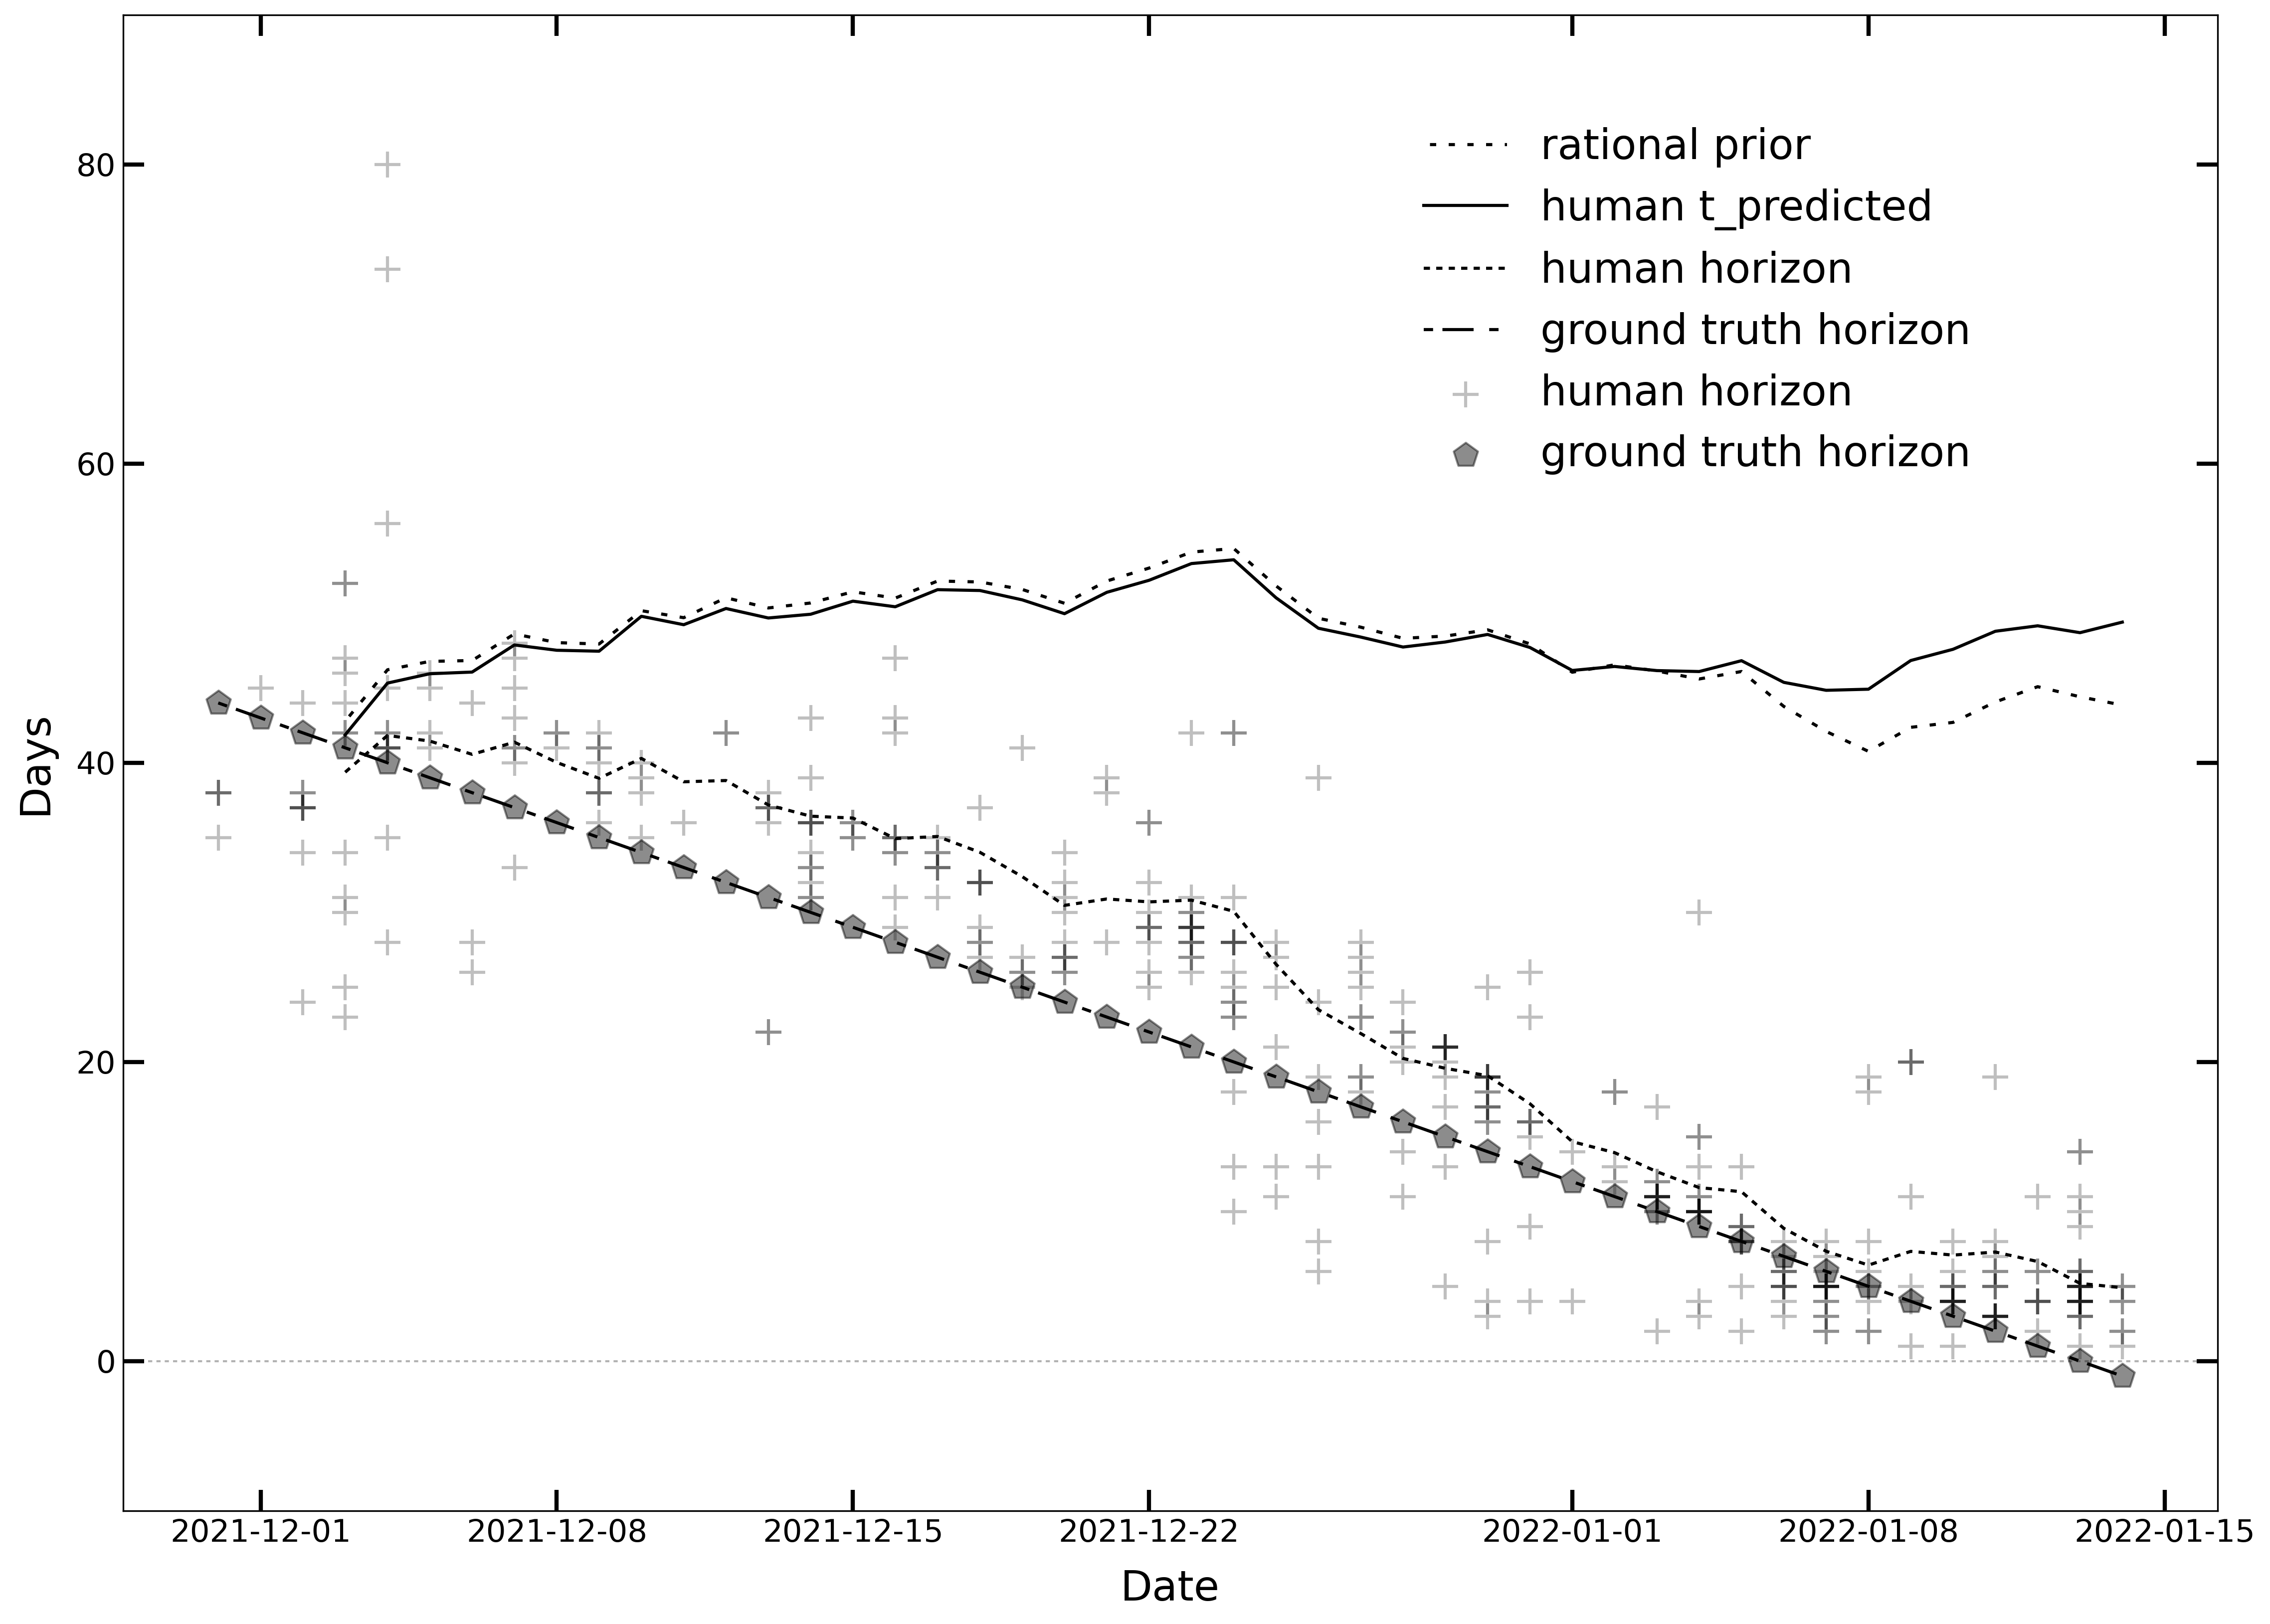
\includegraphics[width=\linewidth]{Figures/Good_all_s.png}
    \caption{The two primary measures, human $t_{predicted}$ and the rational prior (using the median of the recovered prior), over the course of the tournament. (The y-axis shows days; the x-axis shows date of human prediction.)  The human horizon reflects human $t_{predicted}$ minus the date the prediction was generated by the participant.  The ground truth horizon shows the number of days until the actual epidemic peak in Virginia (January 13th, 2022) from each date in the figure; it is the ground truth equivalent of the human horizon.  All trend lines (except the groud truth horizon) were computed as 4-day moving averages. 
    }
    \label{fig:All_Ss_t_tot}
\end{figure}

In terms of the objective of Study 1--to understand the relation between $t_predicted$ and the prior, with emphasis on predictions that have a small horizon--we see in Figure \ref{fig:All_Ss_t_tot} some signature of the predicted \textit{prior crash}, but in attenuated form.  In short, the observations support, provisionally, some middle ground between the two limiting cases that were described in the Introduction (the constant prior vs the constant decision).  The upward trend of the human horizon toward the end of the forecasting window is suggestive of an adaptation on the part of the forecasters as the horizon closes.  

This provisional conclusion is better understood when considering the non-aggregated data (showing all 401 predictions) as shown in Figure \ref{fig:All_S_Scatters}.  In the top-left panel of this figure, we see that the relation between the human predictions and the rational prior are close in value for many of the predictions with a subset of predictions that show larger values for $t_{predicted}$ compared to the prior.  The top-right panel of Figure \ref{fig:All_S_Scatters} shows this result over time, a plot that disaggregates the aggregate figure (Figure \ref{fig:All_Ss_t_tot}) and shows that the difference between a prediction and its prior only manifests near the end of the forecasting window.

The lower two panels in Figure \ref{fig:All_S_Scatters} are the most telling, in terms of the theoretical predictions.  The lower-left figure shows the difference between the human prediction and the prior as a function of the human horizon; it clearly shows that any substantial difference between the two only manifests with human horizons less than 5 days; the lower-right panel shows this result over the forecasting window.  

In summary, Figures \ref{fig:All_Ss_t_tot} and \ref{fig:All_S_Scatters} are suggestive of some adaptation on the part of the participants when the human horizon is small, a suggestion that is more strongly supported by the individual-level data from the most active participants.  We review these data next.

\begin{figure}
    \centering
    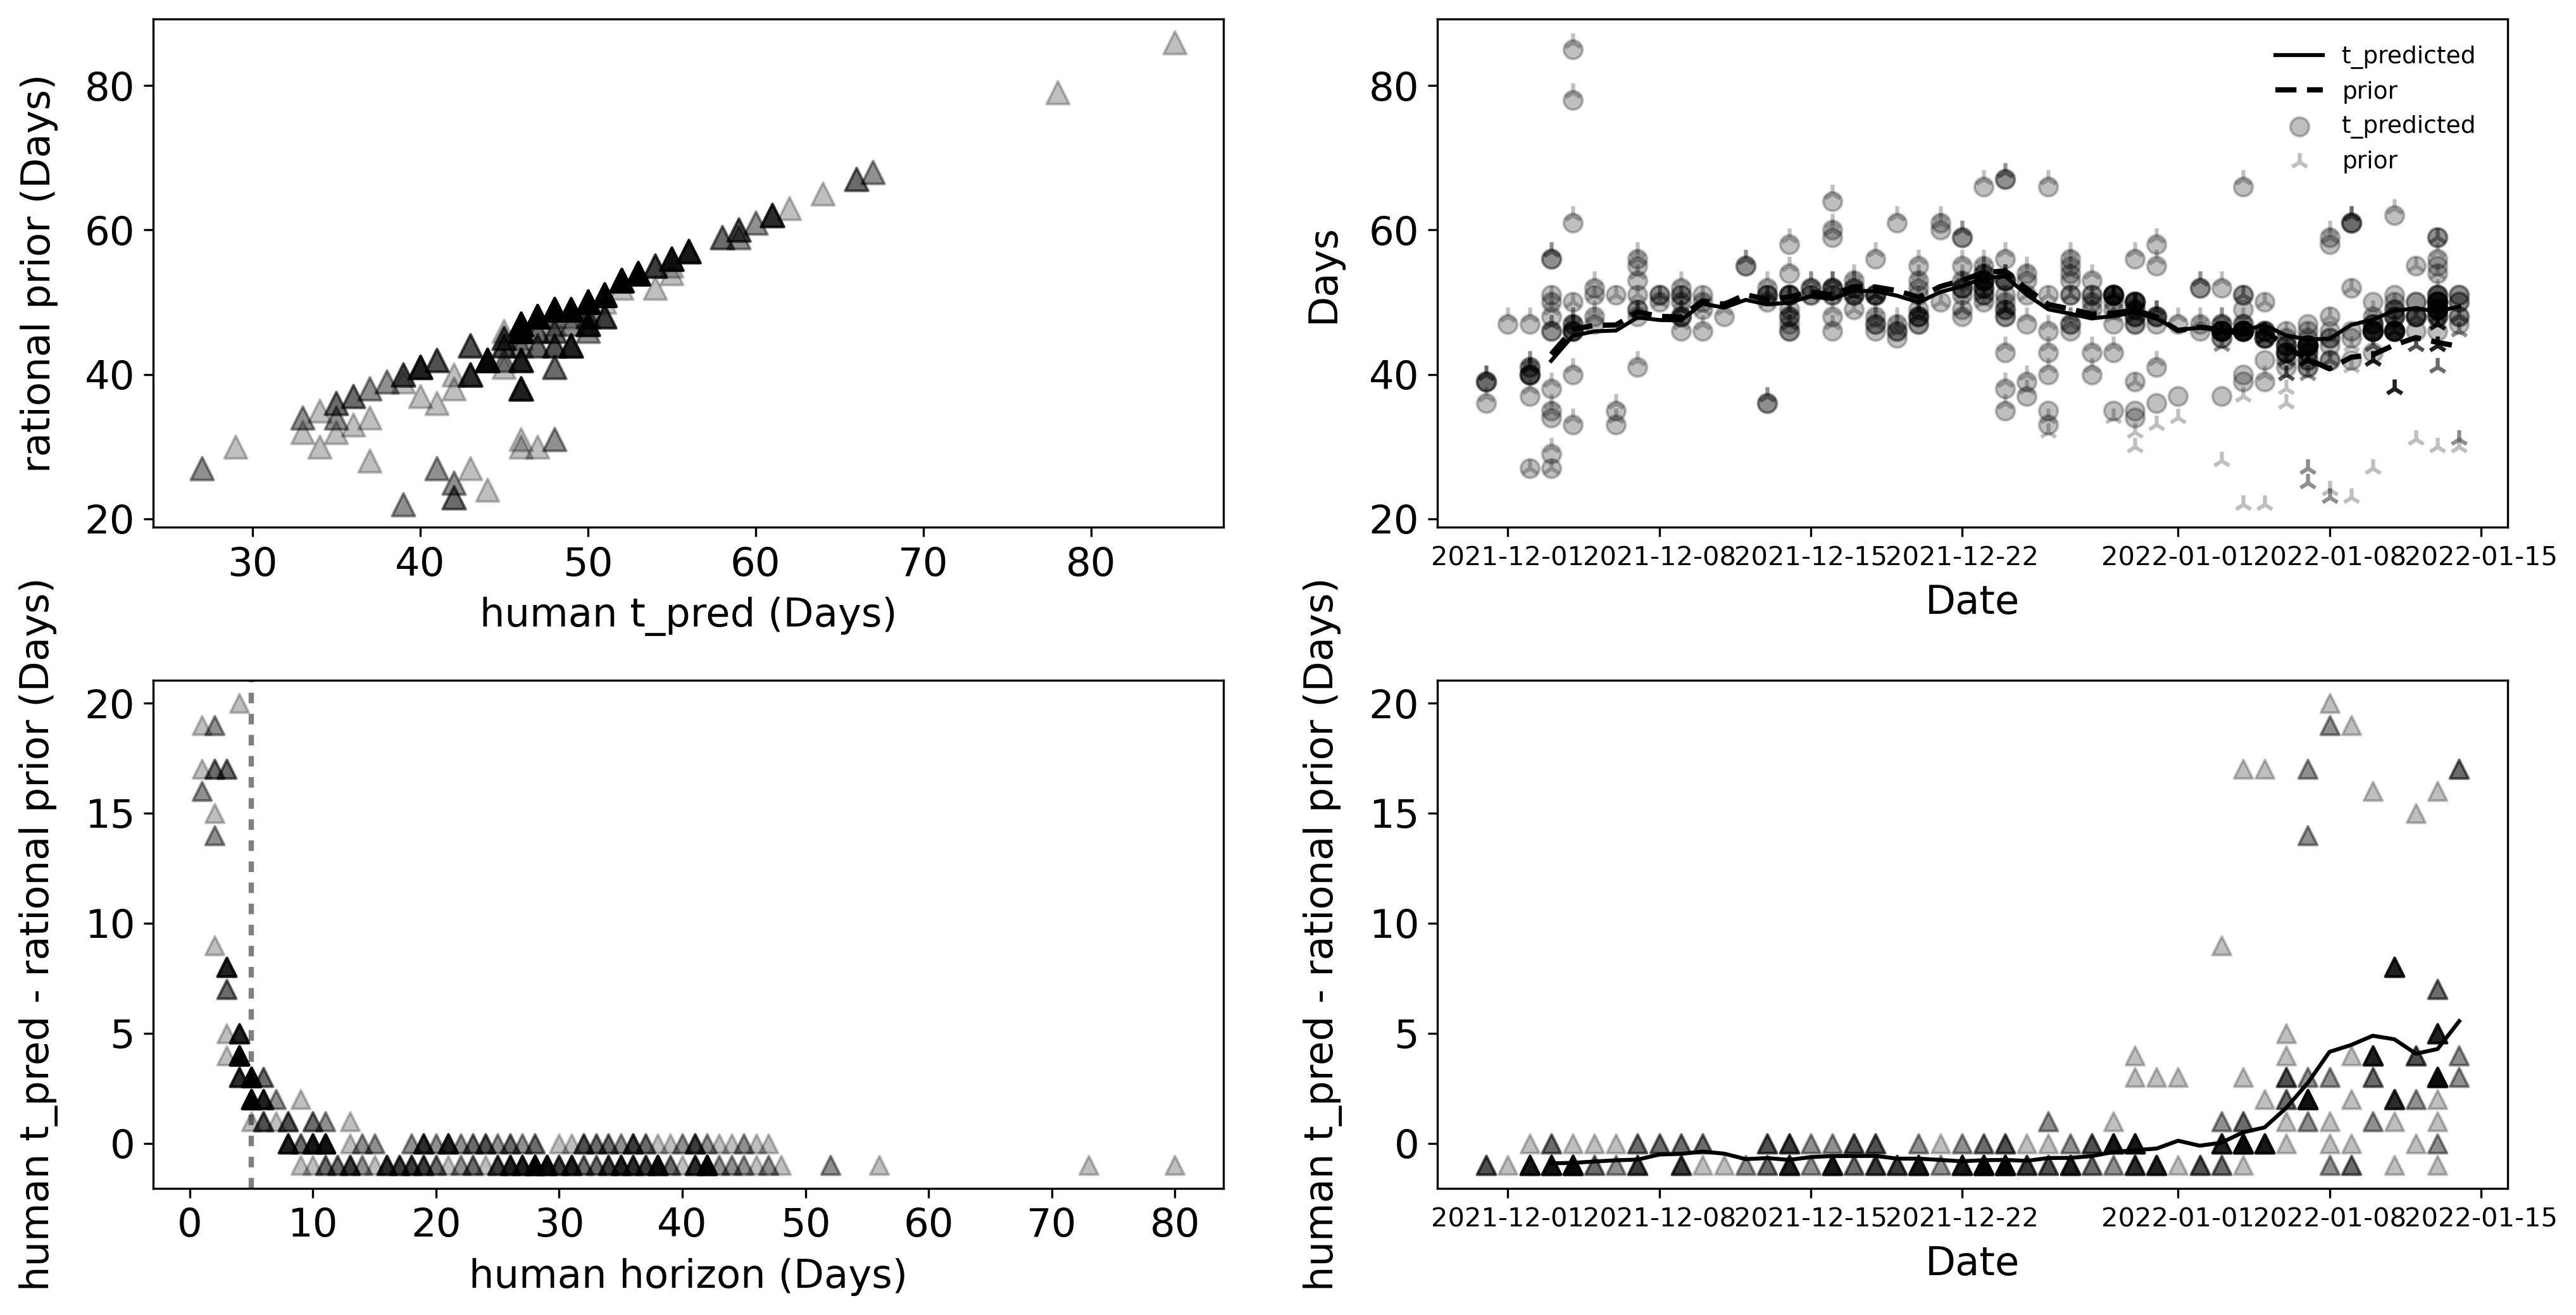
\includegraphics[width=\linewidth]{Figures/Study1_ExplanatoryScatter_All_S.png}
    \caption{The top-left panel shows the relation between the human predictions and the rational prior; The top-right panel shows this relation over time. The lower-left panel shows the difference between the human prediction and the prior as a function of the human horizon; the lower-right panel shows this result over the forecasting window.}
    \label{fig:All_S_Scatters}
\end{figure}

Figure \ref{fig:Single_Ss_t_tot} shows a parallel result to Figure \ref{fig:All_Ss_t_tot} but for the most active subjects (those with more than 15 predictions).  All of the most active participants show some separation of the prior from the human predicted duration of the epidemic, something that is illustrated to a larger degree for participants numbers one, three, five and six.  Further, all of these participants (excepting participant number 4) show the following two signatures of adaptation: an upturn of the predicted duration of the epidemic accompanied by a flattening of the human horizon.  Further analysis of the disaggregated data is shown in Figure \ref{fig:Single_Ss_Summary_2}, a replicate of the lower-right panel of Figure \ref{fig:All_S_Scatters}. For this figure, we added lines that represent the time course for three of the six participants to illustrate the temporal peak of the largest differences between the predicted duration of the epidemic and the prior.  There was a clear peak prior to the end of the prediction window (these are all small horizon predictions, as gathered in the lower-left panel of Figure \ref{fig:All_S_Scatters}) followed by a set of predictions that had a reduced difference between the predicted duration and the prior, likely driven by an increase in the value of $t_{predicted}$.  It is important to note that for each of these three participants, there were multiple predictions both falling within the peak window and post-peak. 

The only participant with large differences between the predicted duration of the epidemic and the prior whom did not show similar behavior was number two; however, this amounts to only only one prediction that peaked for this participant which came very late in the forecasting window.  It is plausible that participant number two would have exhibited a similar signature as the other three participants given time.  The remaining two participants (numbers three and four)  did not exhibit such large differences between their predictions and their recovered priors. 

\begin{figure}
    \centering
    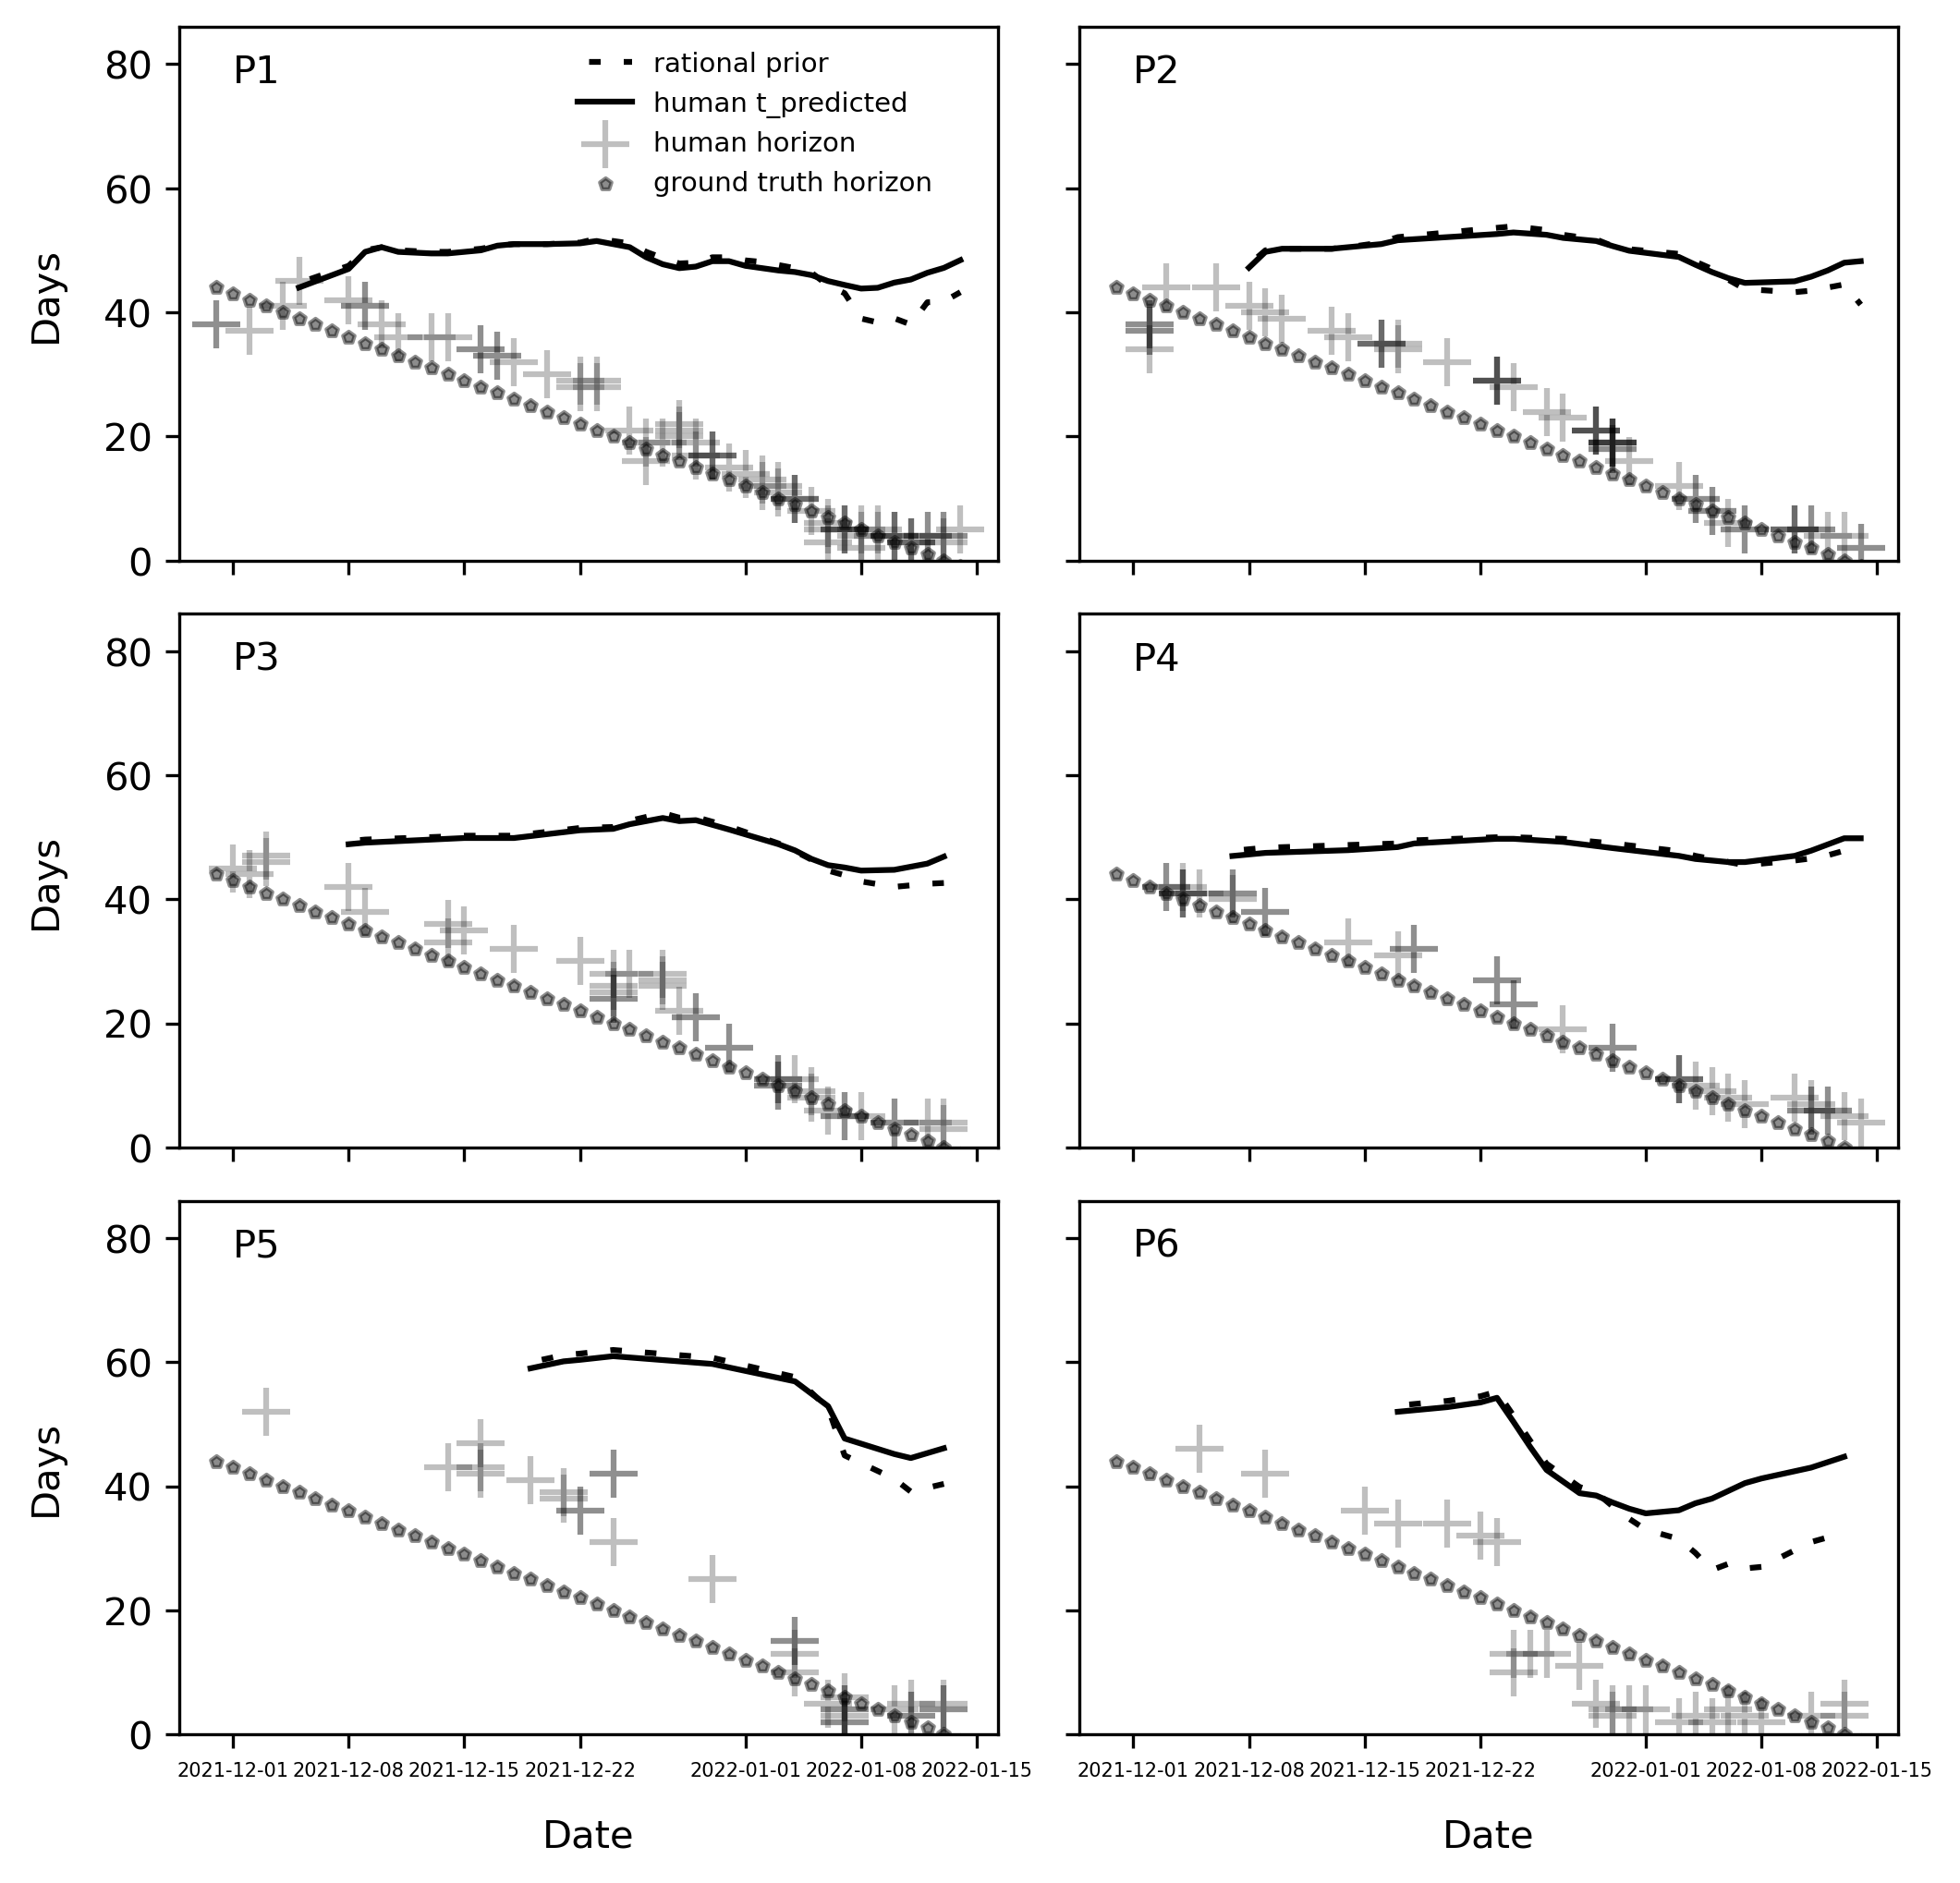
\includegraphics[width=\linewidth]{Figures/Single_Subjects.png}
    \caption{
    This figure depicts the same three components as in Figure \ref{fig:All_Ss_t_tot} for the six subjects with the highest response rate ( $> 15$ responses). Participant number is provided in the top-left corner of each panel.
    }
    \label{fig:Single_Ss_t_tot}
\end{figure}

%%%%%%%
%I DON"T THINK WE NEED THIS FIGURE IT JUST REPLICATES WHAT WE SEE
%WITH ALL Ss
%\begin{figure}
%    \centering
%    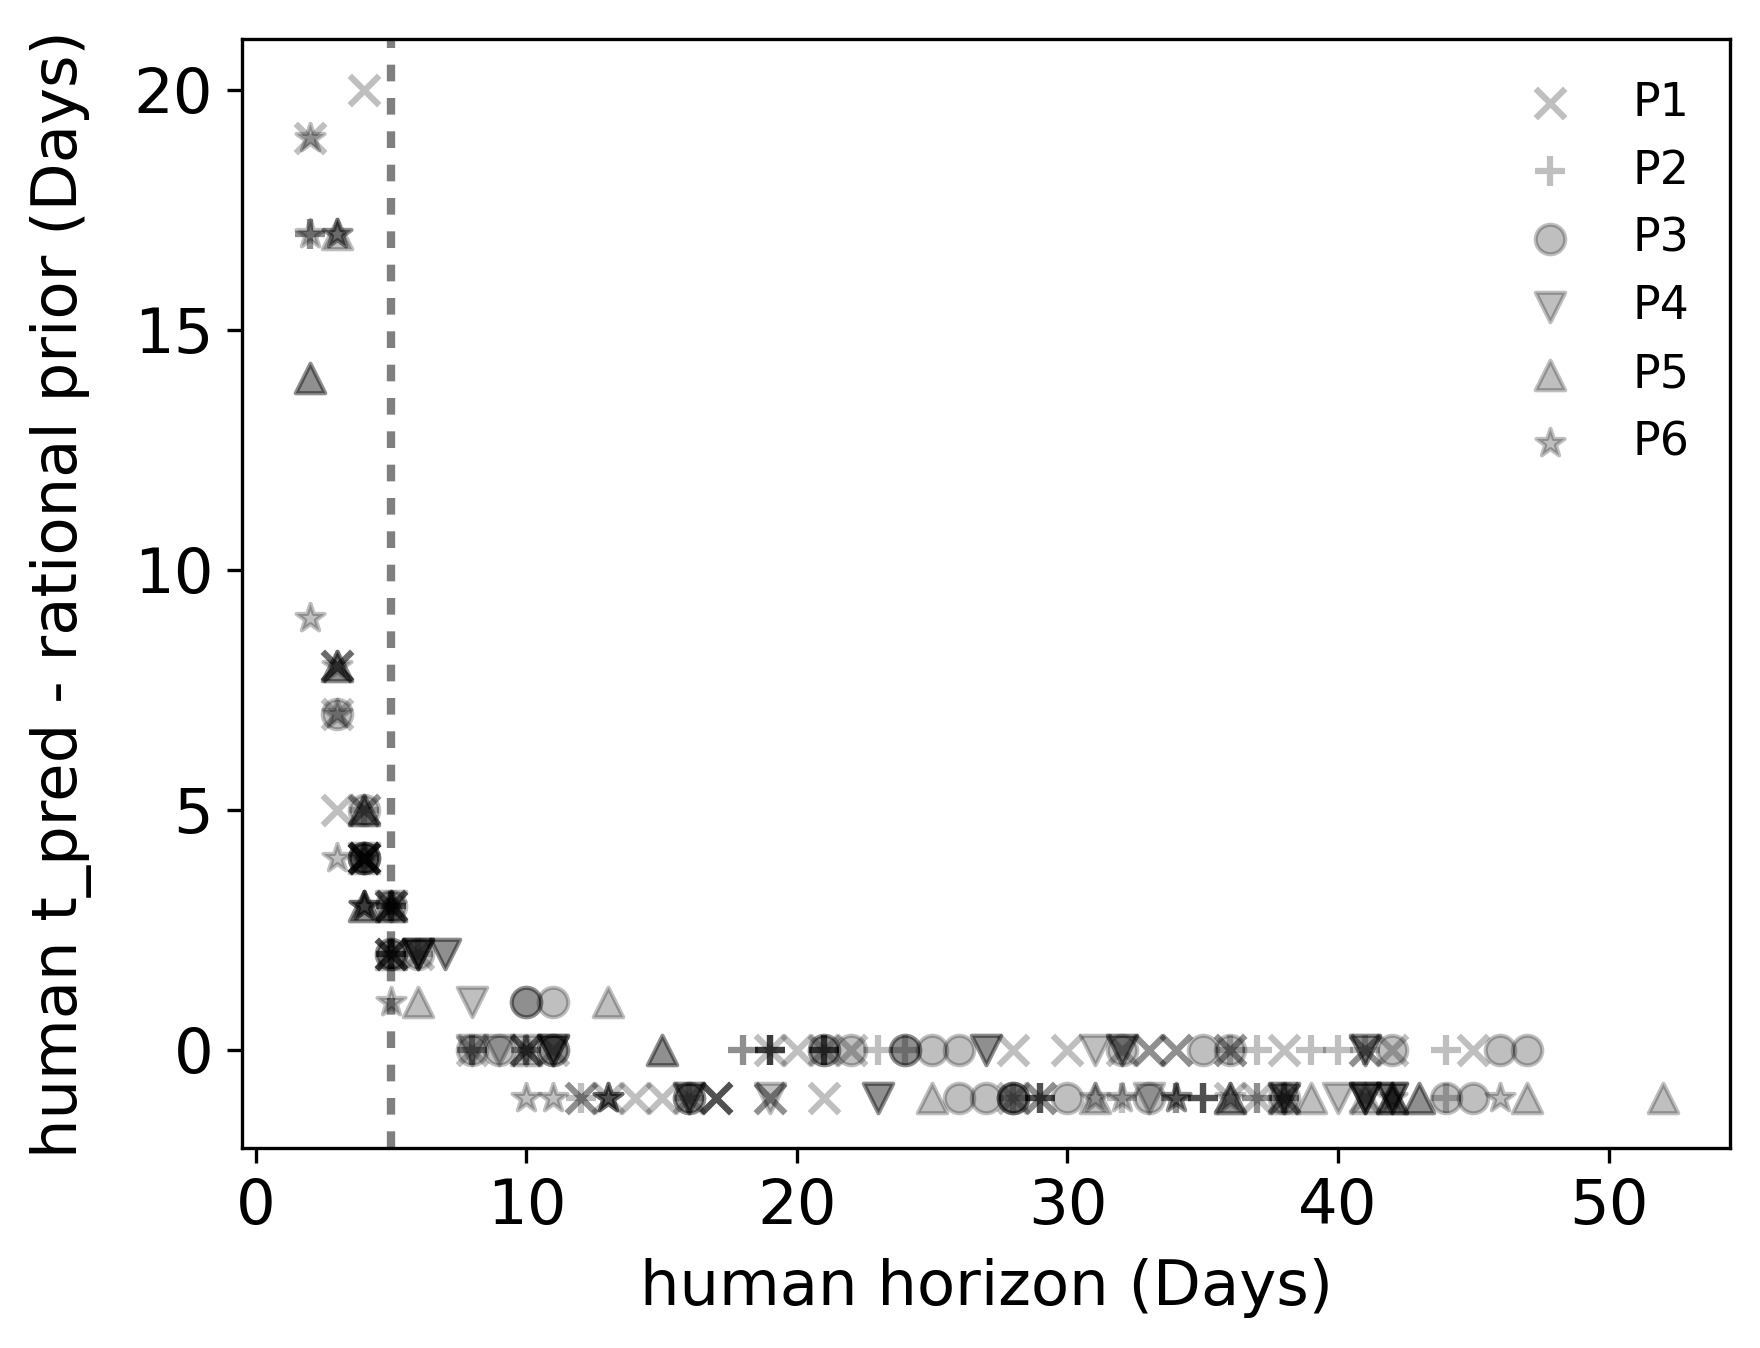
\includegraphics[width=\linewidth]{Figures/Single_Ss_Horiz_Summary.png}
%    \caption{
%    This figure 
%    }
%    \label{fig:Single_Ss_Summary_1}
%\end{figure}

\begin{figure}
    \centering
    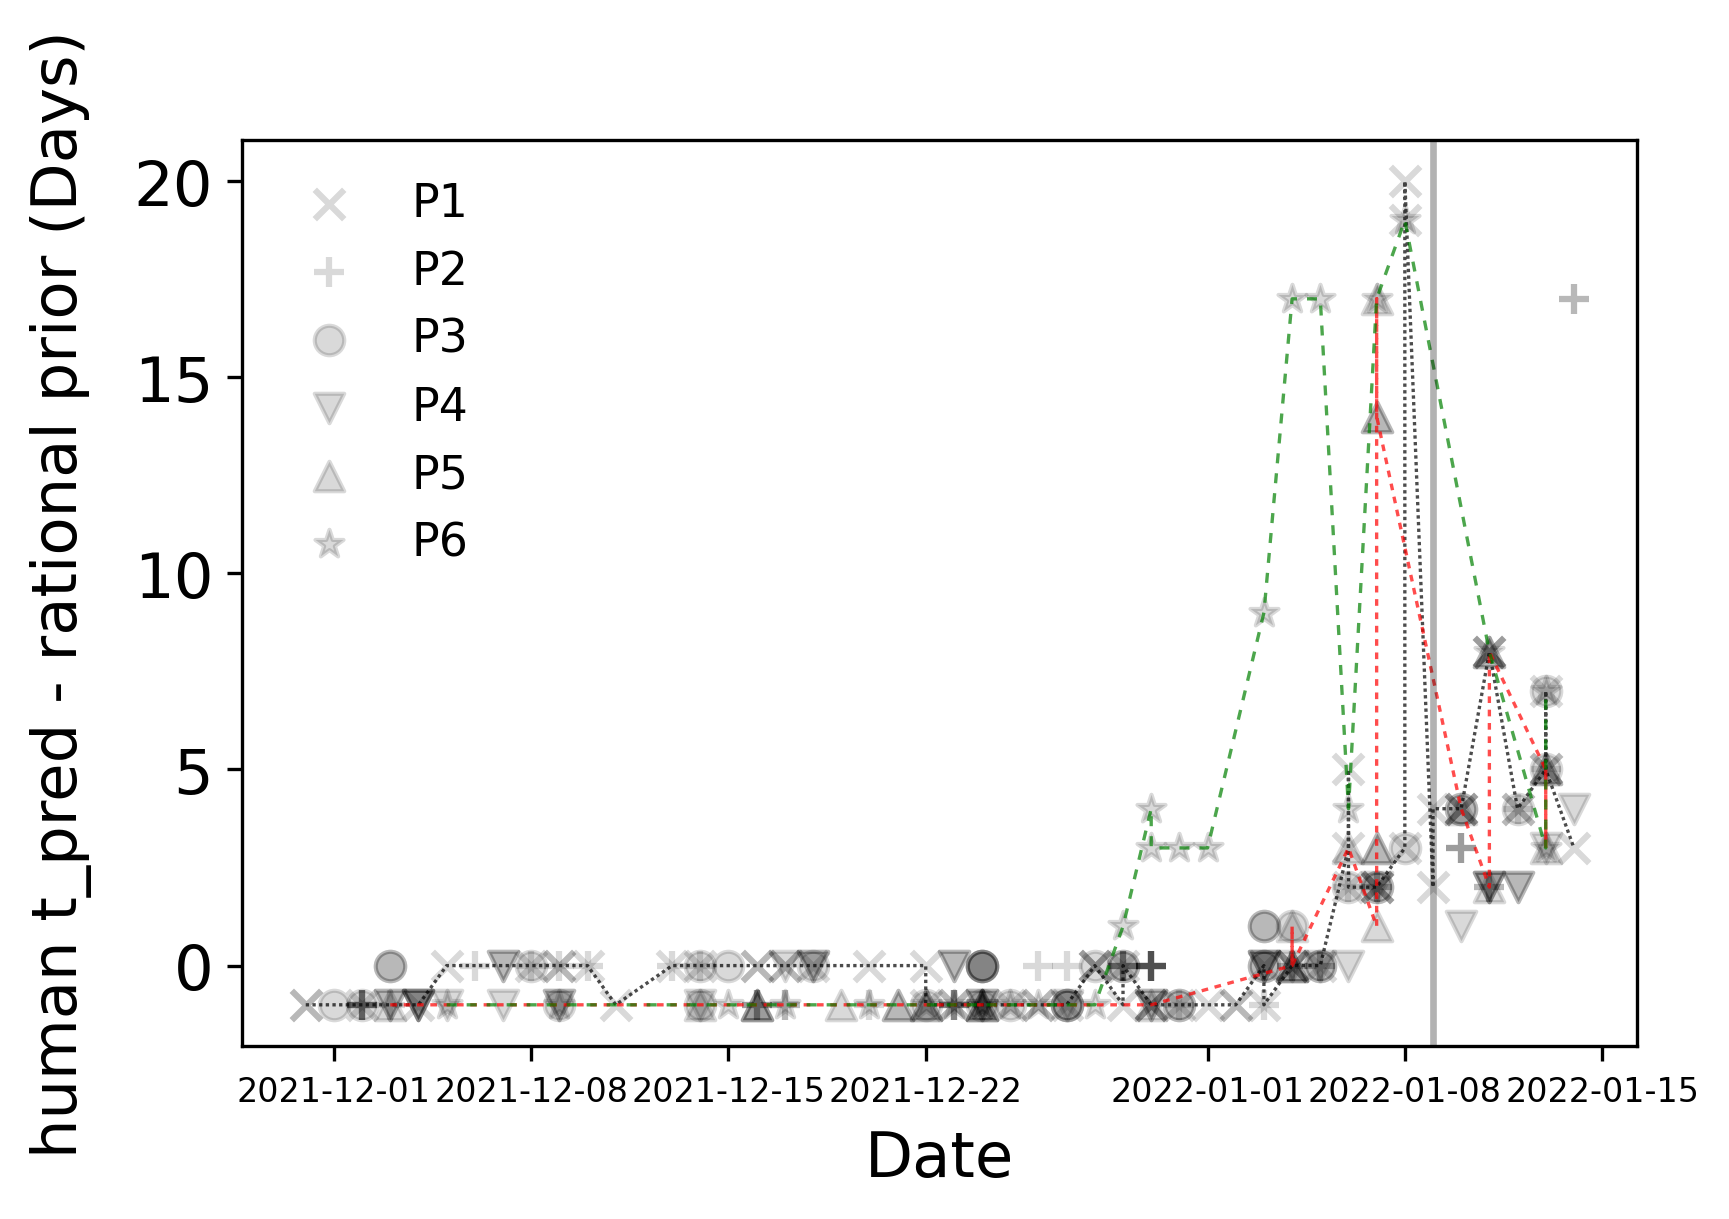
\includegraphics[width=\linewidth]{Figures/Single_Ss_Date_Summary.png}
    \caption{This figure is identical in form to the lower-right panel in \ref{fig:All_S_Scatters}; it shows the six most active participants, each labeled in the figure legend ("P" stands for participant).  The colored, dashed-lines show individual participants (green, participant six; red, participant five; black, participant one). The solid, vertical grey line falls on January 9th, 2022, the date at which (on and after) the predictions for participants one, five and six were post-peak.  See the text for details.}
    \label{fig:Single_Ss_Summary_2}
\end{figure}
